% !TEX encoding = UTF-8 Unicode
% !TEX program = xelatex

\documentclass{article}
	\usepackage[margin = .9in]{geometry}
	\usepackage{fontspec}
	\usepackage{tikz}
	\usepackage{listings}
\begin{document}



	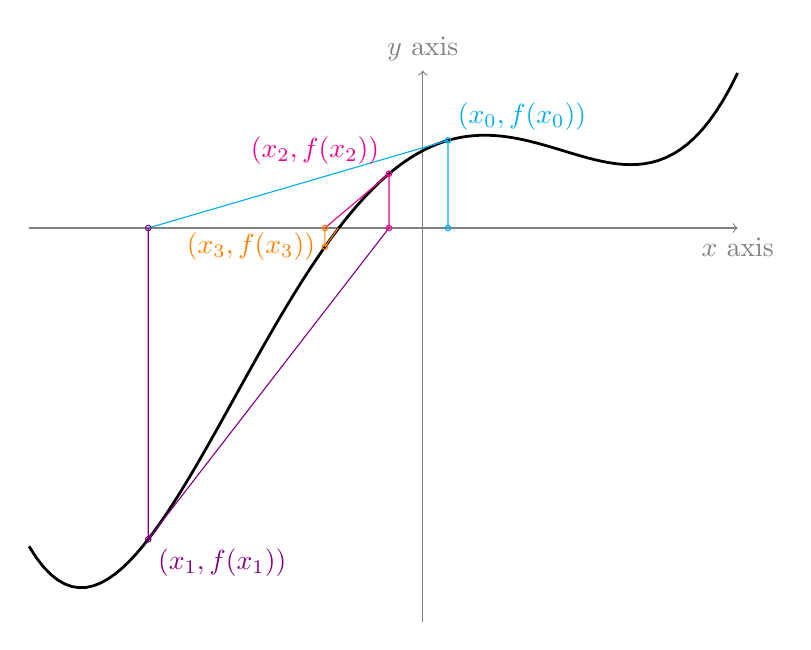
\begin{tikzpicture}
		\draw[gray, ->] (-5, 0) -- (4, 0) node[below]{$x$ axis};
		\draw[gray, ->] (0, -5) -- (0, 2) node[above]{$y$ axis};
		\def\a{1.21} \def\b{-25.6} \def\c{36.1} \def\d{67.8}
		\pgfmathdeclarefunction{f}{1}{\pgfmathparse{
			((#1)^4 + \a*(#1)^3 + \b*(#1)^2 + \c*(#1) + \d)/69}}
		\pgfmathdeclarefunction{dfdx}{1}{\pgfmathparse{
			(4*(#1)^3 + 3*\a*(#1)^2 + 2*\b*(#1) + \c)/69}}
		\draw [line width=1pt] plot
			[variable = \t, domain = -5:4, samples = 100] ({\t}, {f(\t)});
		\pgfmathsetmacro\x{0.321} \pgfmathsetmacro\quo{f(\x)/dfdx(\x)}
		\draw [cyan] ({\x}, 0) circle [radius = 1pt]
			-- ({\x}, {f(\x)}) circle [radius = 1pt]
				node [above right] {$(x_0, f(x_0))$}
			-- ({\x - \quo}, {0});
		\pgfmathsetmacro\x{\x-\quo} \pgfmathsetmacro\quo{f(\x)/dfdx(\x)}
		\draw [violet] ({\x}, {0}) circle [radius = 1pt]
			-- ({\x}, {f(\x)}) circle [radius = 1pt]
				node [below right] {$(x_1, f(x_1))$}
			-- ({\x - \quo}, {0});
		\pgfmathsetmacro\x{\x-\quo} \pgfmathsetmacro\quo{f(\x)/dfdx(\x)}
		\draw [magenta] ({\x}, {0}) circle [radius = 1pt]
			-- ({\x}, {f(\x)}) circle [radius = 1pt]
				node [above left] {$(x_2, f(x_2))$}
			-- ({\x - \quo}, {0});
		\pgfmathsetmacro\x{\x-\quo} \pgfmathsetmacro\quo{f(\x)/dfdx(\x)}
		\draw [orange] ({\x}, {0}) circle [radius = 1pt]
			-- ({\x}, {f(\x)}) circle [radius = 1pt]
				node [left] {$(x_3, f(x_3))$}
			-- ({\x - \quo}, {0});
	\end{tikzpicture}



	\fontspec{SourceCodePro-Regular}
	\lstset{
		language=[latex]tex, tabsize=4,
		moredelim=*[s][\itshape]{$}{$},
		moredelim=*[s][\color{red!40!.}]{(}{)},
		moredelim=*[s][\color{green!30!.}]{[}{]},
		backgroundcolor=\color{blue!5},
		commentstyle=\color{.!80}\itshape,
		texcsstyle=*\color{blue!40!.},
		moretexcs={
			draw,pgfmathsetmacro,pgfmathdeclarefunction
		},
		deletetexcs={},
	}
	\lstinputlisting{math3.tex}

\end{document}